\section{September 2023: LibrePCB 1.0.0}

\begin{frame}{\secname}
  \begin{itemize}
    \item<1-> Advanced PCB features (thermal reliefs, blind \& buried vias, slotted pads, \ldots)
    \item<2-> 3D PCB viewer \& STEP export
    \item<3-> Assembly variants \& MPN management
      \begin{itemize}
        \item Adding MPNs to libraries
        \item Specifying MPNs in schematics
        \item Alternate (second-source) MPNs
        \item Different parts in each assembly variant
        \item Separate BOM for each assembly variant
      \end{itemize}
    \item<4-> Output jobs
      \begin{itemize}
        \item Unified export for any kind of production data
        \item Highly customizable
        \item 100\% reproducible/portable
        \item Runnable from GUI and CLI
      \end{itemize}
  \end{itemize}

  \begin{tikzpicture}[remember picture,overlay]
    \node<1>[xshift=0cm,yshift=-0.5cm] at (current page.center){%
    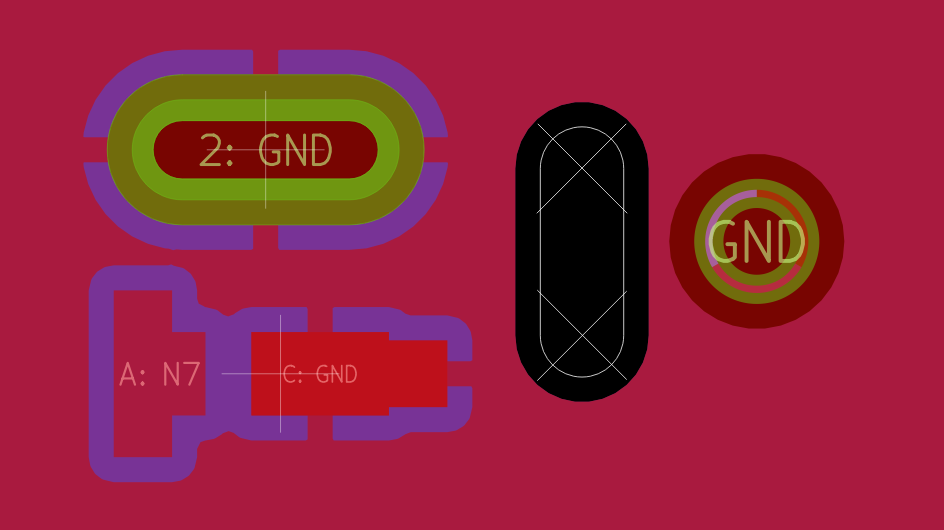
\includegraphics[height=5.5cm]{images/advanced_features.png}};

    \node<2>[xshift=0cm,yshift=-1cm] at (current page.center){%
    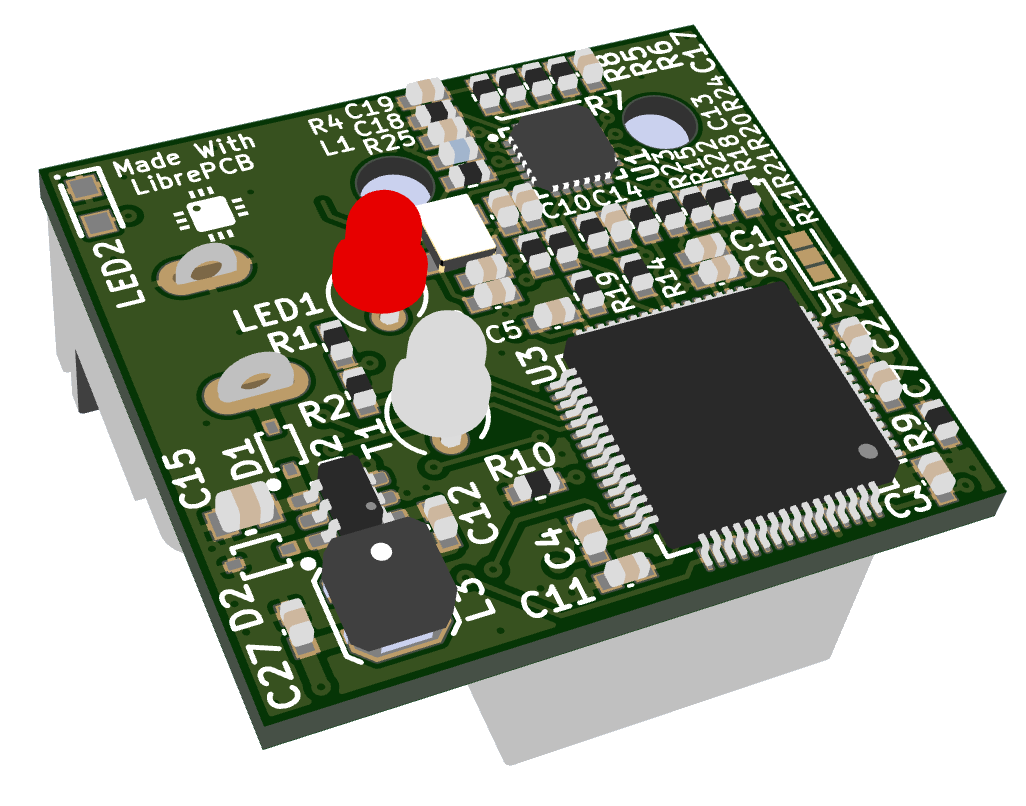
\includegraphics[width=8cm]{images/3d_viewer.png}};

    \node<3>[xshift=0cm,yshift=-2.5cm] at (current page.center){%
    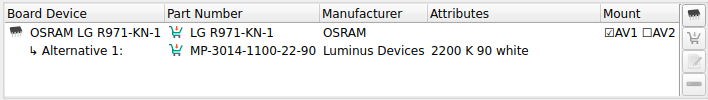
\includegraphics[width=13.5cm]{images/mpn_management.png}};

    \node<4>[xshift=4.9cm,yshift=-0.8cm] at (current page.center){%
    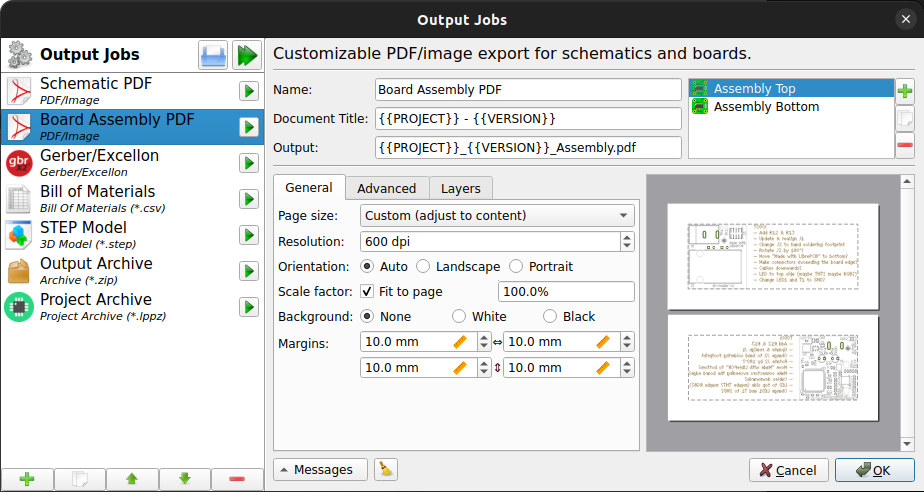
\includegraphics[trim=0 0 9.9cm 0,clip,height=5.5cm]{images/output_jobs.png}};
  \end{tikzpicture}
\end{frame}
